% Sample Paper for Poster Conference
%( without guarantee:-)) 
%send your comment to xrund@fel.cvut.cz
%
\documentclass{ibws_template}
% 
%----------------------------------------------------------
%             THIS IS THE PLACE FOR YOUR FAVORITE PACKAGES
%
%\usepackage[latin2]{inputenc}%
%\usepackage{babel}%
%\usepackage{czech}%
\usepackage[utf8]{inputenc}
\usepackage[english,czech]{babel}
%\usepackage{psfrag}
%\usepackage{amsmath}
%\usepackage{pifont,amssymb}
\addto\captionsenglish{\renewcommand{\figurename}{Fig.}}


\begin{document}
%----------------------------------------------------------

%----------------------------------------------------------
%               THIS IS THE PLACE OF THE TITLE
%
\title{AROM: Autonomous robotic observatory manager}
%----------------------------------------------------------
%               THIS IS THE PLACE FOR THE AUTHORS NAMES AND THE TITLE FOR HEADINGS
%
\headtitle{R. Dvořák, J. Kákona, J. Štrobl; AROM: Autonomous robotic observatory manager}
%----------------------------------------------------------
%               THIS IS THE PLACE FOR THE AUTHORS NAMES - ALL AUTHORS MUST HAVE A STUDENT STATUS!!!

%
\author{Roman Dvořák\affiliationmark{1}, Jakub Kákona \affiliationmark{1,2}, Jan Štrobl \affiliationmark{3}}
%----------------------------------------------------------
%              THIS IS THE PLACE FOR AFFILIATIONS
%
\affiliation{%
\affiliationmark{1} MLAB, Czech Republic, roman-dvorak@email.cz \\
\affiliationmark{2} CTU Prague, Czech Republic, kakonjak@fel.cvut.cz\\
\affiliationmark{3} Astronomical Institute of the Czech Academy of Sciences, strobl@asu.cas.cz
}
%--------------------------------------------------------------


\maketitle

%----------------------------------------------------------
%               THIS IS THE PLACE FOR ABSTRACT

\begin{abstract}\\
AROM (Autonomous robotic observatory manager) is a set of open-source software for the control and management of robotic observatories. The whole software is built upon a system for controlling robots - ROS (Robotic operation system).

AROM software is designed for use with small (amateur) telescopes and fully autonomous observatories and is going to work on simple single-board computers like Odroid. Software should be able to monitor all telescope states which may affect observing quality. These conditions include weather, air quality, observatory status, mount position and many others.
\end{abstract}


%----------------------------------------------------------
%               THIS IS THE PLACE FOR KEYWORDS
\begin{keywords}
Robotic telescope, observatory, ROS, networking, TCP/IP, open-source, automation.
\end{keywords}

%----------------------------------------------------------
%               HERE WRITE YOUR PAPER

\section{Introduction}
There are few systems for controlling robotic telescopes. Some of them are commercial and expensive. They are usually custom-made for a specific installation. Besides that, there exist a few open-source (or free) systems which do not meet the requirements for all applications - for most part, they are not able to control the observatory in a fully autonomous mode.

\section{Goals}
The goals of this project are based on personal experience with observing and testing other systems.

Main goals are as follows:
\begin{itemize}
\item Minimal maintenance requirements
\item Independent on control computer
\item Serviceless observing (robotic observing)
\item Self-calibration, self-diagnostics
\item Price affordability
\item Simple and intuitive operation
\item Multiple telescope observing
\item Open-source software, easily expandable
\end{itemize}

It should also be noted that the aim of the project is to provide a solution that enables the observer to care only for observations, not for hardware or software problems. Besides that, the management software also contains many useful tools for observing itself.


\subsection{Observing scheduler}
Scheduler is used to define observing plan. It can optimize the observing plan in order to make use of the full observing times with the best conditions for target objects. Such conditions include observing near meridians, shorter slewing or calculation of object rise and set times. Every target can have a defined set of observing conditions like the minimum height above horizon, list of measuring times etc.
\subsection{Observing script}
Observing script defines parameters for capturing data from instruments. It must be a part of observing because it tells which device to use and how. For example „use the main camera with the exposure time of 20 seconds“ or „use video-guiding with the second camera and change filter between every image or try to refocus the main camera if necessary“.

It can also contain algorithms for capturing HDR (high dynamics range) images, wide-field mosaics or calibration images (flat-field, dark-frame, bias).


\subsection{Movement limits}
Movement limits represent a safety mechanism to avoid telescope crash to observatory walls, roof or other pieces of equipment. There are two limit levels: the first one represents artificial horizon, i. e. the area covered by trees or distant buildings. In the first level restrictions the telescope can slew, while the second level delimit restricted areas where there is a danger of the telescope crashing. The area of movement limits are defined by means of a vector image (.svg).

\subsection{Astrometry}
Astrometry is a method for star position measurement. It can be used to accurately measure the position of a telescope and finetuning the errors caused by GoTo movements.


\subsection{Alignment and guiding}
Alignment tells us how accurately the polar axis of the mount is established. Usually, it contains calibrating process, which determines differences of mount coordinates and real coordinates at three points. This process may be replaced with astrometry and permanent guiding.

Guiding is used for restriction of mount mechanical errors as periodic error or some mechanical deformations. It can replace standard alignment workflow and make it continuously.

\subsection{User interface}
User interface enables to the user comfortably controlling telescope and all devices. AROM user interface is main based web page which intuitively shows device state and drive options. It configuration of whole observatory assembly.

\begin{figure}[h!]
\begin{center}
  \selectlanguage{english}
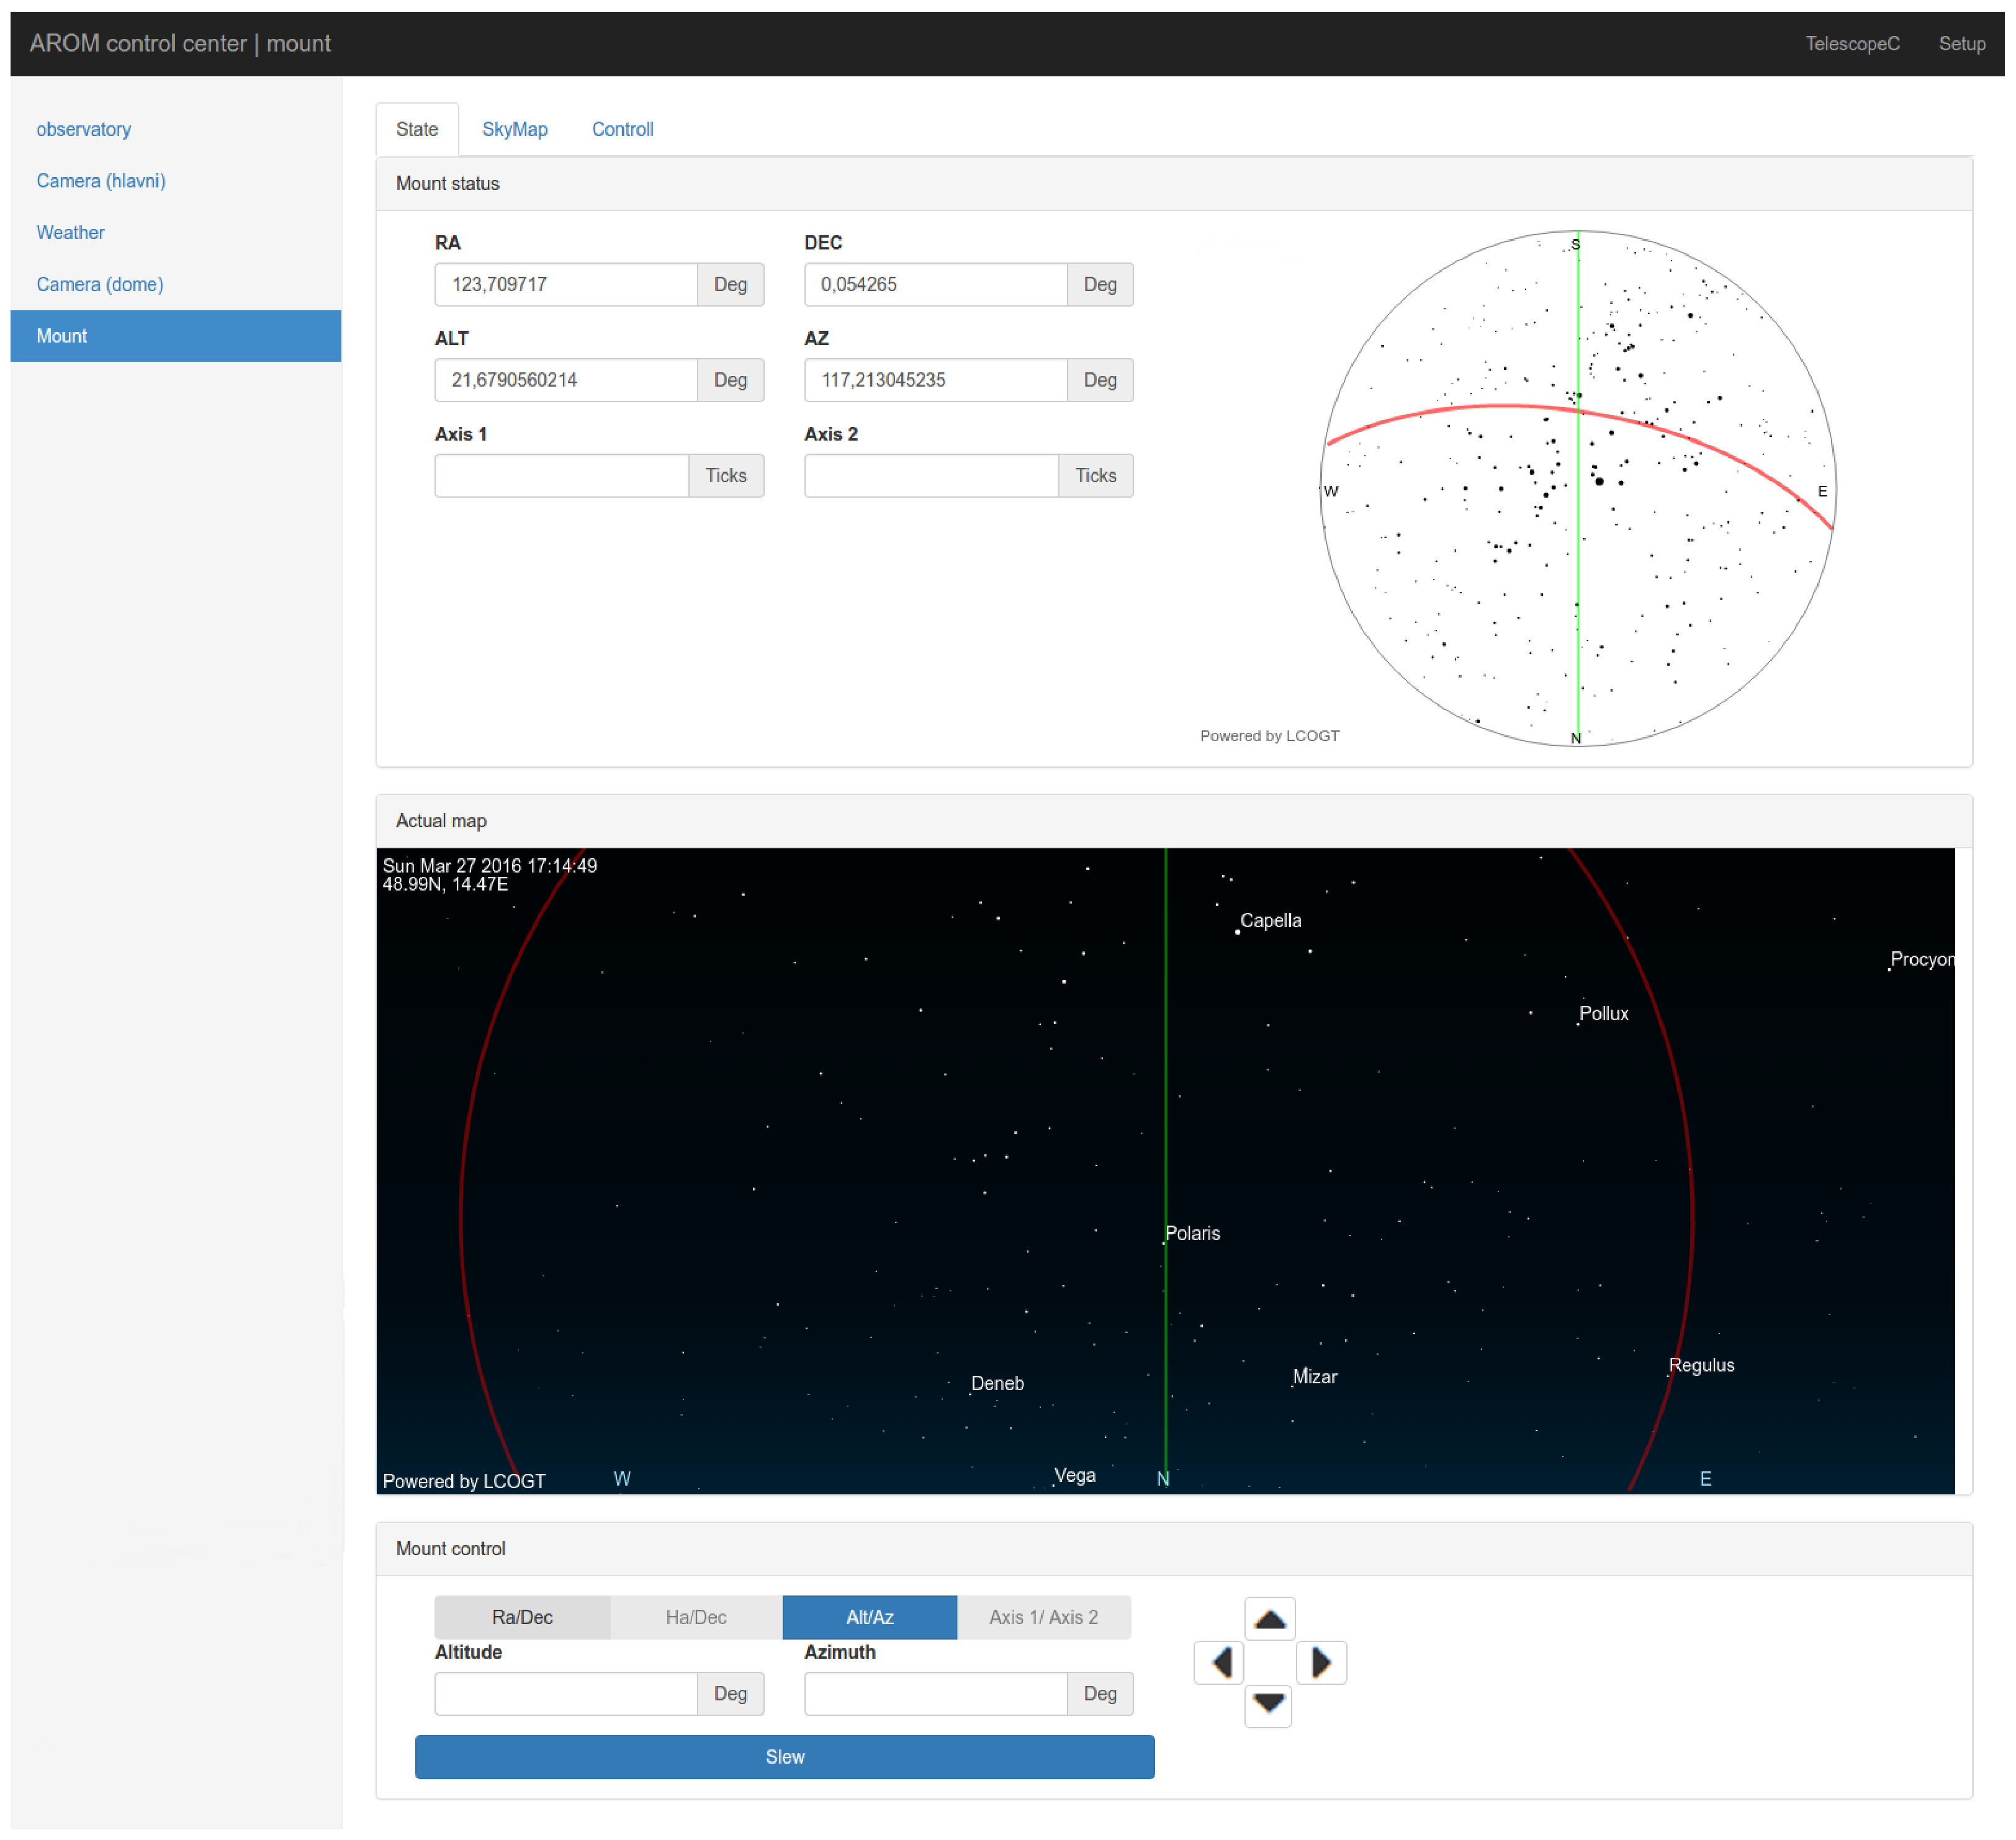
\includegraphics[width=72mm]{img/arom_ui.eps}
\caption{AROM control web page; mount overview.} 
\end{center}
\end{figure}
\pagebreak

Web user interface has the advantage in platform independence. Observer can control it from the computer only with web browser or via smart phone. 

The second important user interface is in a terminal. This type of remote control is useful in the cases of remote control via internet without public IP address or in networks with low transfer rate. Terminal user interface offers to the users full control without visual content as showing captured fields, sky map or stream from overview cameras.

\subsubsection{Control modes}
AROM will have three main control modes. First mode is the fully autonomous mode. It requires fully equipped observatory with a closable roof, weather station, cloud sensor, back-up batteries and more. Telescope is going to observe without any user interaction. It will observe object with pre-set object list and it will chose best target object. 

The second mode is manual mode. This mode is designed for use with free-standing telescope systems. The user specifies targets and system controls camera by own. AROM keeping the correct position specified by user.

The third mode is semi-automatic mode. This mode is automatic mode designed for free-standing telescopes. This mode requires operator for weather monitoring. Capturing of images is controlled by 'Observing scheduler' and 'Observing scripts'.

\section{ROS}
ROS is set of software tools for controlling robotic systems. For AROM is very important TCP/IP messaging system. TCP/IP messaging system provides communication between nodes. Node is a program which can communicate with other nodes. There are several types of messages. 

The first type of messages must have topic (name of message) and data. This message is created by publisher (node) on topic and received by subscriber with listening the same topic. This type of message can have more publishers and subscribers (N-N).

The second type of messages (services) is send from node to the specified node with same topic (N-1). After sending first message. The publisher will wait for answer. It is useful for getting state of the node.

The last type (activities) is designed for longer processes as some mechanical moving or long-running calculations. This message is non-blocking.

\pagebreak
\section{AROM structure}
Software structure is designed to use ROS system. The main part of the software is the master node 'AROM\_brain'. Master node contains parametric server where values describing telescope, cameras, observing site, and other parameters are stored. 

In AROM scheme is every hardware device controlled by own node. Nodes are connected in hierarchical structure.

The hierarchical structure is important. The structure defines devices dependencies. For example we have a camera. Camera can move with focuser, field rotator, filter wheel or some other camera's equipment. These devices are controllable only from camera driver (node). This structure ensures independent controlling of the more same devices. see \texttt{Fig. 2}.
 
There are exist nodes, which can not be included in hierarchical structure. These are observatory state monitor node, guiding node, software for validating image, software for saving images to the network storage, etc.

Some data as weather condition could be shared through network from another AROM setup.

\subsection{Configuration}
Structure should be defined in observatory .xml configuration file. Here is described every device used in setup. This file is useful for automatic starting of system. Device drivers (nodes) could be also loaded/killed later.


\begin{figure}[b!]
\begin{center}
  \selectlanguage{english}
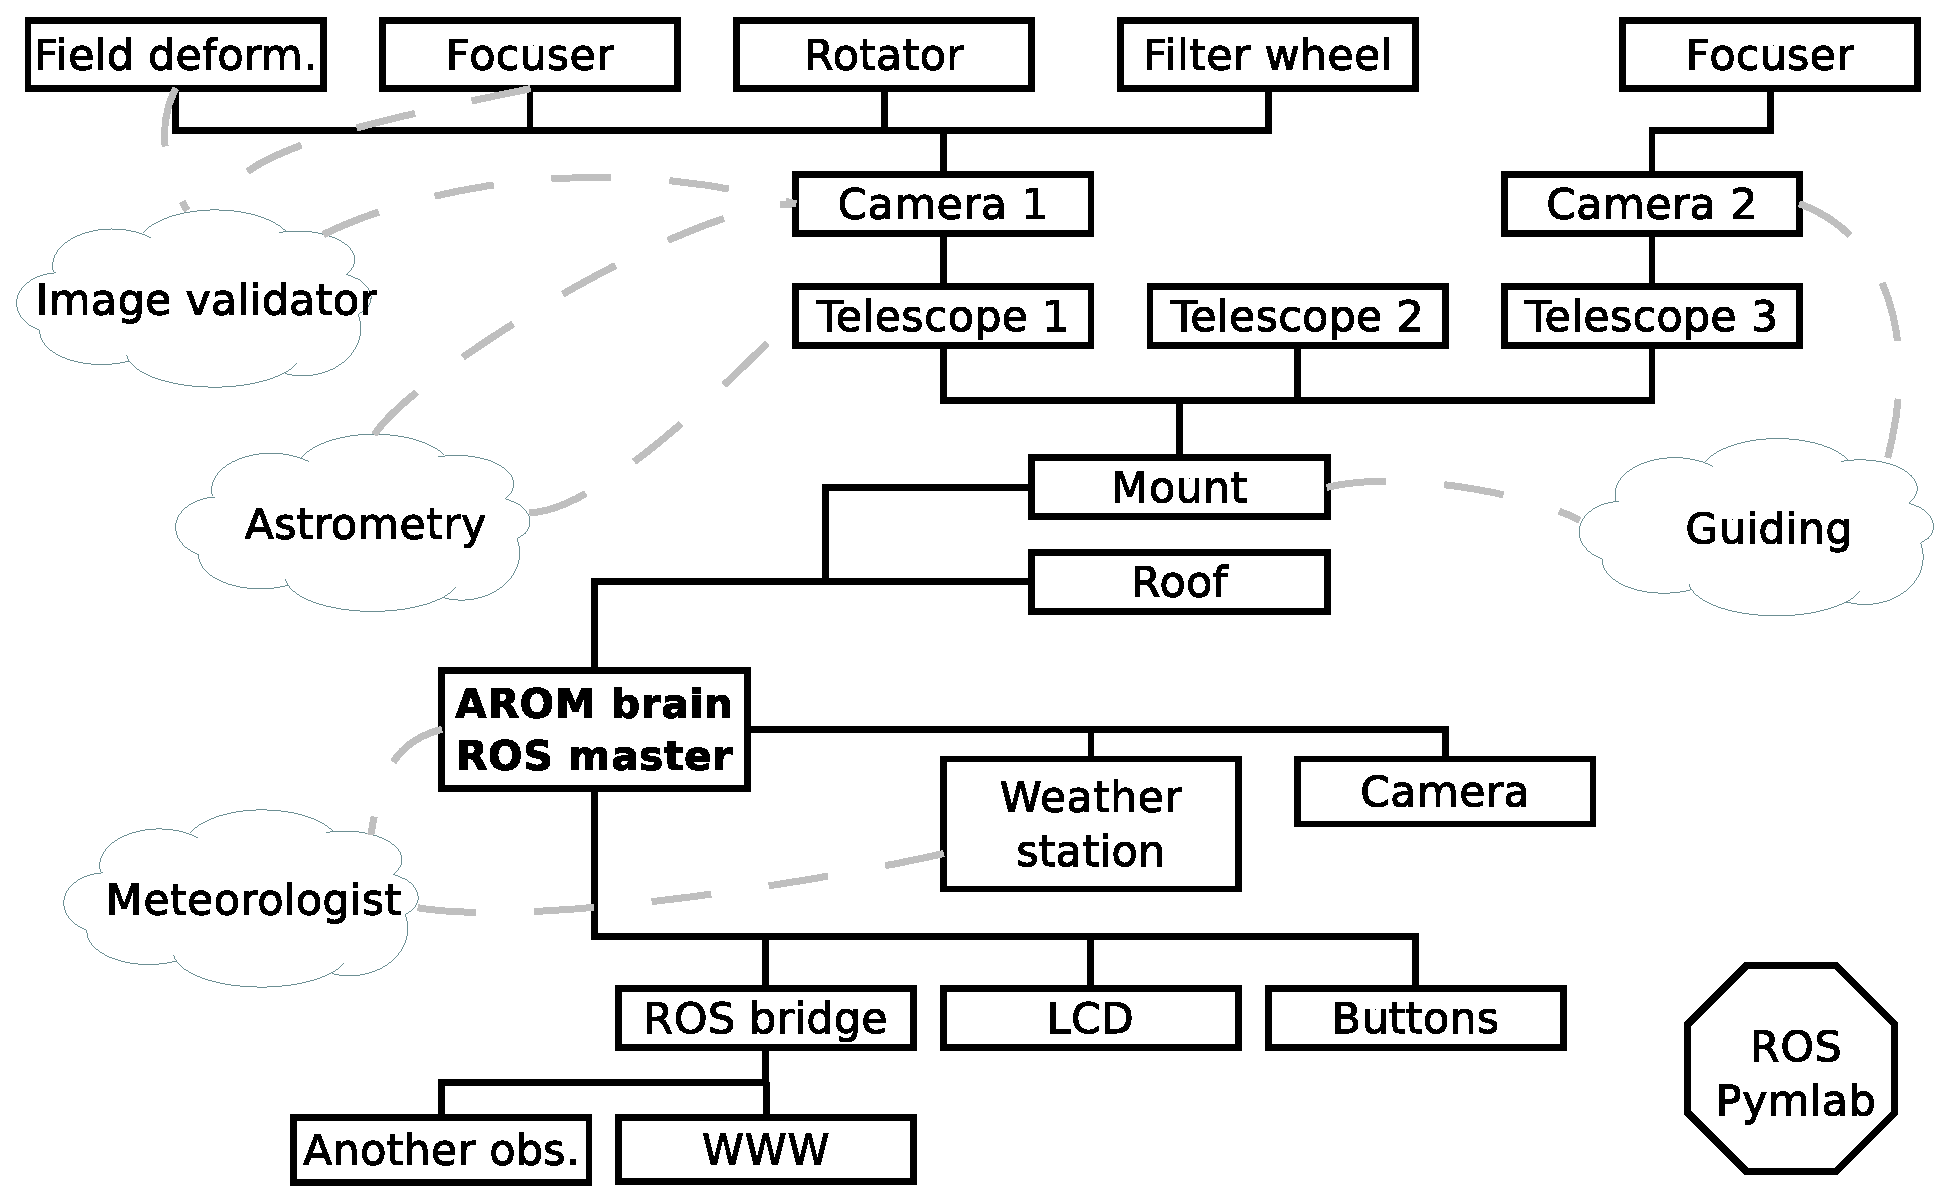
\includegraphics[width=160mm, height=91mm]{img/ros_structuce.eps}
\caption{Schema of AROM drivers (ros nodes).} 
\end{center}
\end{figure}


\section{Database}
All system requires database for storage data as weather during the observation, catalogue of objects, observed data, observation logs, observing scripts. Database can be shared between multiple observatories. Database is be based on MySQL framework.

Object database must be able to save multiple types of objects as stars, planets, comets, asteroids, satellites, etc. Example of database structure for storing object is shown in table \texttt{Table 1.}

\begin{table}[h]
\begin{center}
  \selectlanguage{english}
{\renewcommand{\arraystretch}{1.8}
\tablefont
\begin{tabular}{|c|c|c|c|}
\hline
Name
&Type
&Example 1
&Example 2\\
\hline
\hline
id
&int
&0
&1\\
\hline
name
&varchar
&CC Lyn
&C/2014 Q2\\
\hline
name\_other
&varchar
&SAO 41877
&Lovejoy\\
\hline
name\_cat
&varchar
&HD 60335
&Null\\
\hline
author
&int
&0
&2\\
\hline
type
&decimal
&1.234
&5.2\\
\hline
ra
&decimal
&113.98325
&Null\\
\hline
dec
&decimal
&+43.03097
&Null\\
\hline
other
&varchar
&Null
&[Orbital Elements]\\
\hline
describe
&varchar
&V* EW type
&Terry Lovejoy\\
\hline
\end{tabular}}
\caption{Example of structure of table 'objects'.}
\label{tab}
\end{center}
\end{table}
\vspace{11cm}

%----------------------------------------------------------
%               HERE IS EXAMPLE OF A FIGURE	
%		environment {figure} for one-column figure, {figure*} for two-column figure 
%	 	\caption{} for one-column caption, \captionwide{} for two-column figure
%
%\begin{figure}[ht!]
%\begin{center}
%\resizebox{65mm}{!}{\includegraphics{obr1.eps}}
%%\input{obr/dr1a.pstex_t}
%\caption{AROM software structure \texttt{Obrázek1}.
%} 
%\label{figs}
%\end{center}
%\end{figure}%\vspace{5mm}

\section{Safety system}
Safety system is the most important part of whole system. It protect equipment from the destruction. Damage may be caused by many circumstances, such as as crash telescope into other observatory equipment or damage camera by high temperature. This system may prevent even just dust on optical parts. 

\section{Conclusion}
Even today in the time of the various technology there is no well usable system for robotization various small observatories or amateur telescopes. AROM is prides on openness, simply extensibility, support of various hardware, and intuitiveness for operator. AROM allows control of simple free-standing telescope setups as well as complex observatories. AROM system could be used also on the radiotelescopes.

%----------------------------------------------------------
%               THIS IS THE PLACE FOR  ACKNOWLEDGEMENTS
%\section*{Acknowledgements}


%----------------------------------------------------------
%               THIS IS THE PLACE FOR REFERENCES
\begin{thebibliography}{9}

\bibitem{paper} Downey. E. C., \emph{INDI: Instrument-Neutral Distributed Interface}, 2007 [Online], March 2016

\bibitem{paper} Monet. D. G. et al, 2003, \emph{The USNO-B Catalog}, The Astronomical Journal 125 984–993.

\bibitem{} Kubánek P., \emph{RTS2 - The Remote Telescope System}, Advances in Astronomy, vol. 2010, Article ID 902484, 9 pages, 2010

\bibitem{}University of Göttingen, "RTML - Remote Telescope Markup Language", [online], April 2016

\end{thebibliography}



%----------------------------------------------------------
%               THIS IS THE PLACE FOR AUTHOR CV
%\begin{authorcv}{Roman DVOŘÁK} He is 18 years old student of high school in České Budějovice. He is interested in astronomy, robotics and modern technologies. 

%\end{authorcv}

\end{document}

